\chapter{Objets physiques de haut niveau}\label{chapter-HLO}

\section{Introduction}\label{chapter-HTT_analysis-section-introduction}

Citer \fullcite{CMS-PAS-HIG-17-020}

et aussi nouvelle version full runII si possible

+ HIG-14-029, HIG-13-021


Citer la thèse de Gaël:\\\fullcite{Gael_thesis}

Citer également la thèse d'Artur?\\\fullcite{Artur_thesis}


Études déjà menées au LEP~\cite{Schael:2006cr} et au Tevatron~\cite{Aaltonen:2009vf,Abazov:2011jh}

LHC: \cite{CMS-PAS-HIG-13-021,CMS-PAS-HIG-14-029,CMS-PAS-HIG-17-020}

aussi avec \quarkb\antiquarkb~\cite{Chatrchyan:2013qga,Khachatryan:2015tra}

ATLAS \mu\mu\ et \tau\tau~\cite{Aad:2012cfr,ATLAS-MSSM-HTT_2018,ATLAS-MSSM-HTT_2020}

CMS \mu\mu~\cite{CMS:2015ooa} \tau\tau~\cite{Chatrchyan:2012vp,CMS-MSSM-HTT_2014,CMS-PAS-HIG-17-020}


données réelles, simulées et encapsulées  -> appendix
seulement quatre canaux, pas six
$L_1$, $L_2$

what were my tasks?

	
Artur Il Darovic Gottmann
12:26
Homework concerning the bbH and ggH samples?
12:28




1) Monitor the production ---> ask in case there are invalid samples
2) Process the new samples
3) Rederive the ggH weights based on input POWHEG samples
4) Update the signal modelling for new samples in CombineHarvester
rwolf profile image	
Roger Wolf
12:32
And on the experimental side I recall:
newes FF's
MET tail correction and uncertainty
Are these the only items left before wrapping up or am I missing anything in addition?

\subsection{Énergie transverse manquante}\label{chapter-LHC-section-evt_reco-subsec-MET}
Des particules neutres interagissant peu avec le détecteur, en particulier les neutrinos, peuvent être produites lors des collisions et se propager sans laisser de signal dans le détecteur, les rendant ainsi invisibles.
Toutefois, lorsque de telles particules sont produites en association avec des particules détectées, leur présence peut être déduite du déséquilibre dans le moment total des particules de l'événement~\cite{CMS-PAS-JME-17-001}.
\par Les collisions de protons, dont la phénoménologie est discutée section~\ref{chapter-LHC-section-LHC-subsec-pp_collisions}, présentent une impulsion totale dans le plan transverse nulle dans l'état initial.
Par conservation, l'impulsion totale dans le plan transverse est nulle dans l'état final.
La somme des impulsions transverses des particules invisibles doit donc compenser celle des particules reconstruites, \ie
\begin{equation}
\sum_{\substack{\text{toutes les}\\\text{particules}}} \vpT = \vec{0}
\Leftrightarrow
\sum_{\substack{\text{particules}\\\text{invisibles}}} \vpT + \sum_{\substack{\text{particules}\\\text{reconstruites}}} \vpT = \vec{0}
\Leftrightarrow
\sum_{\substack{\text{particules}\\\text{invisibles}}} \vpT = -\sum_{\substack{\text{particules}\\\text{reconstruites}}} \vpT \mend
\end{equation}
\par L'énergie transverse manquante (MET, \emph{Missing Transverse Momentum}) est ainsi définie comme
\begin{equation}
\vMET = -\sum_{\substack{\text{particules}\\\text{reconstruites}}} \vpT
\msep
\MET = \abs{\vMET}
\mend[,]
\end{equation}
et représente l'impulsion transverse totale des particules invisibles.
Cette définition correspond à la MET \og brute \fg{} (\emph{raw MET}) et doit être corrigée des effets de reconstruction de l'événement.
C'est en particulier le cas lors de la calibration en énergie des jets, ce qui est abordé dans le chapitre~\refChJERC.


\subsection{Formation des jets}\label{chapter-MSSM-formation_jets}
Lorsqu'un parton (quark ou gluon) est issu d'une collision de particules, il possède une haute énergie et émet alors, par interaction forte, d'autres partons.
Par conservation, l'énergie portée par chaque parton ainsi obtenu diminue et par conséquent, $\alpha_s$ augmente.
\par Tant que l'échelle d'énergie est suffisamment grande pour que $\alpha_s \ll 1$, ce qui correspond à des énergies supérieures à la centaine de \SI{}{\MeV}, il est possible de réaliser des calculs perturbatifs.
L'émission de partons créé la \og gerbe partonique \fg, sujet de la prochaine section.
\par Au fur et à mesure des émissions, l'échelle en énergie diminue et en deçà d'une centaine de \SI{}{\MeV}, il n'est plus possible de réaliser des calculs perturbatifs car $\alpha_s$ augmente.
Des modèles paramétriques sont alors utilisés pour caractériser le phénomène d'\og hadronisation \fg, abordés ensuite.

\subsubsection{Gerbe partonique}\label{chapter-MSSM-formation_jets-subsec-gerbe-partonique}
%\fullcite{Unorthodox_Introduction_QCD}
Lorsqu'un parton est issu d'une collision au LHC, il se trouve dans un premier temps dans le régime de liberté asymptotique. Il émet alors d'autres partons. Ainsi, pour un événement $\Zboson\to\quark\antiquark$ comme celui de la figure~\ref{subfig-fgraph-Z_q_q} avec deux quarks dans l'état final, il est possible d'obtenir par émission d'un gluon un état $\quark\antiquark\gluon$ comme ceux illustrés sur les figures~\ref{subfig-fgraph-Z_qg_q} et~\ref{subfig-fgraph-Z_q_qg}, par exemple.
\begin{figure}[h]
\centering\vspace{\baselineskip}
\subcaptionbox{\label{subfig-fgraph-Z_q_q}}[.3\textwidth]
{\begin{fmffile}{Z_q_q}\fmfstraight
\begin{fmfchar*}(30,20)
  \fmfleft{i}
  \fmfright{o1,o3}
  \fmf{boson, tension=2}{i,v1}
  \fmf{phantom}{o1,v1,o3}
  \fmffreeze
  \fmf{fermion}{o1,v1,o3}
  \fmflabel{\Zboson}{i}
  \fmflabel{\quark}{o3}
  \fmflabel{\antiquark}{o1}
  \fmfdot{v1}
\end{fmfchar*}
\end{fmffile}
\vspace{\baselineskip}}
\hfill
\subcaptionbox{\label{subfig-fgraph-Z_qg_q}}[.3\textwidth]
{\begin{fmffile}{Z_qq_q}\fmfstraight
\begin{fmfchar*}(30,20)
  \fmfleft{i}
  \fmfright{o1,o2,o0,o3}
  \fmf{boson, tension=2}{i,v1}
  \fmf{phantom}{o1,v1,o3}
  \fmffreeze
  \fmf{fermion}{o1,v2,v1,o3}
  \fmffreeze
  \fmf{gluon}{v2,o2}
  \fmflabel{\gluon}{o2}
  \fmflabel{\Zboson}{i}
  \fmflabel{\quark}{o3}
  \fmflabel{\antiquark}{o1}
  \fmfdot{v1,v2}
\end{fmfchar*}
\end{fmffile}
\vspace{\baselineskip}}
\hfill
\subcaptionbox{\label{subfig-fgraph-Z_q_qg}}[.3\textwidth]
{\input{\PhDthesisdir/plots_and_images/Feynman_diagrams/gerbe_partonique/fgraph-Z_q_qg.tex}\vspace{\baselineskip}}
\caption[Un boson \Zboson\ se désintègre en paire quark-antiquark.]{Un boson \Zboson\ se désintègre en paire quark-antiquark. Dans les cas des figures~\ref{subfig-fgraph-Z_qg_q} et~\ref{subfig-fgraph-Z_q_qg}, un gluon supplémentaire est émis.}
\label{fig-fgraph-Z_q_q_xg}
\end{figure}
\par Il est légitime de se demander quelle est la probabilité d'obtenir un état $\quark\antiquark\gluon$ à partir d'un état $\quark\antiquark$.
Des calculs de section efficace permettent d'obtenir~\cite{salam2010elements}, pour un état initialement à $X$ partons dont un parton $i$ émet un parton $j$,
\begin{equation}
\dd{\sigma_{X+j}} \simeq \sigma_{X} \sum_{i\in\set{X}} \frac{\alpha_s}{2\pi} \frac{\dd{\theta^2}}{\theta^2} \dd{z} P_{ij}(z)
\end{equation}
où $\theta$ est l'angle entre le parton émis $j$ et le parton émetteur $i$. La grandeur $P_{ij}(z)$ est la probabilité qu'un parton de type $i$ émette un parton de type $j$ emportant une fraction $z$ de l'énergie initiale de $i$, qui s'exprime
\begin{align}
P_{\quark\quark}(z) &= C_F \frac{1+z^2}{1-z} \msep&
P_{\quark\gluon}(z) &= C_F \frac{1+(1-z)^2}{z} \mend[,]
\\
P_{\gluon\gluon}(z) &= C_A \frac{z^4 + 1 + (1-z)^4}{z(1-z)} \msep&
P_{\gluon\quark}(z) &= T_R (z^2+(1-z)^2) \mend[,]
\end{align}
et $P_{\gluon\antiquark}(z) = P_{\gluon\quark}(z)$,
avec
$C_F=\frac{4}{3}$,
$C_A = 3$ et
$T_R=\frac{1}{2}$.
La probabilité d'émettre un parton supplémentaire diverge dans deux cas:
\begin{itemize}
\item le parton émis a une énergie faible devant celle du parton émetteur, c'est la limite infrarouge;
\item l'angle entre le parton émis et le parton émetteur est petit, c'est la limite colinéaire.
\end{itemize}
\par Les nouveaux partons ainsi émis et les partons initiaux continuent chacun ce processus jusqu'à ce que le phénomène de confinement de couleur réapparaisse. Pour un unique parton directement issu de la collision ayant lieu au vertex primaire (PV), une gerbe partonique est formée, \ie\ un ensemble collimé de partons, comme illustré sur la figure~\ref{fig-parton_shower}.
Ce sont ces particules qui vont participer au phénomène d'hadronisation dû au confinement de couleur.
\begin{figure}[h]
\centering
\subcaptionbox{Deux quarks sont initialement produits, ce qui correspond au diagramme de la figure~\ref{subfig-fgraph-Z_q_q}.\label{subfig-parton_shower-qq}}[.3\textwidth]
{\begin{tikzpicture}
\def\Lenght{2.5}
\def\qangle{45}
\def\antiqangle{\qangle+180}

\clip (-\Lenght,-\Lenght) rectangle (\Lenght,\Lenght) ;

\fill (0,0) circle (2pt);
\draw (0,0) node [left] {PV} ;

\draw (0,0) --+ (\qangle:\Lenght) node [left] {\quark} ;
\draw (0,0) --+ (\antiqangle:\Lenght) node [right] {\antiquark} ;


\end{tikzpicture}}
\hfill
\subcaptionbox{Un des quarks peut émettre un gluon, ce qui correspond au diagramme de la figure~\ref{subfig-fgraph-Z_q_qg}.\label{subfig-parton_shower-qqg}}[.3\textwidth]
{\begin{tikzpicture}
\def\Lenght{2.5}
\def\qangle{45}
\def\antiqangle{\qangle+180}

\clip (-\Lenght,-\Lenght) rectangle (\Lenght,\Lenght) ;

\fill (0,0) circle (2pt);
\draw (0,0) node [left] {PV} ;

\draw (0,0) --+ (\qangle:\Lenght) node [left] {\quark} ;
\draw (0,0) --+ (\antiqangle:\Lenght) node [right] {\antiquark} ;


\def\Lfrac{3}
\draw (0,0) --+ (\qangle:\Lenght/\Lfrac) coordinate (g1) ;
\draw (g1) + (\qangle-30:\Lenght-\Lenght/\Lfrac) coordinate (g2) ;
\draw [decoration={aspect=0.6, segment length=1.75mm, amplitude=1mm,coil},decorate] (g2) -- (g1) ;

\end{tikzpicture}}
\hfill
\subcaptionbox{Le processus est réitéré, donnant un ensemble de particules colorées.\label{subfig-parton_shower-qqNg}}[.3\textwidth]
{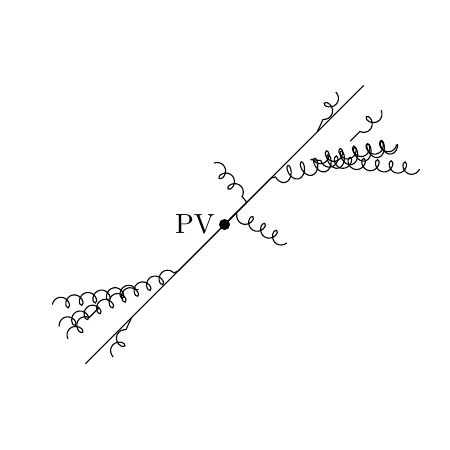
\begin{tikzpicture}
\def\Lenght{2.5}
\def\qangle{45}
\def\antiqangle{\qangle+180}

\clip (-\Lenght,-\Lenght) rectangle (\Lenght,\Lenght) ;

\fill (0,0) circle (2pt);
\draw (0,0) node [left] {PV} ;

\draw (0,0) --+ (\qangle:\Lenght) node [left] {\quark} ;
\draw (0,0) --+ (\antiqangle:\Lenght) node [right] {\antiquark} ;


\def\Lfrac{3}
\draw (0,0) --+ (\qangle:\Lenght/\Lfrac) coordinate (g1) ;
\draw (g1) + (\qangle-30:\Lenght-\Lenght/\Lfrac) coordinate (g2) ;
\draw [decoration={aspect=0.6, segment length=1.75mm, amplitude=1mm,coil},decorate] (g2) -- (g1) ;

\draw (g1) + (\qangle-20:{(\Lenght-\Lenght/\Lfrac)/(\Lfrac/2)}) coordinate (g3) ;
\draw (g3) + (\qangle:{\Lenght-\Lenght/\Lfrac-(\Lenght-\Lenght/\Lfrac)/(\Lfrac/2)}) coordinate (g4) ;
\draw [decoration={aspect=0.8, segment length=1.75mm, amplitude=.75mm,coil},decorate] (g4) -- (g3) ;

\draw (g1) + (\qangle-20:{(\Lenght-\Lenght/\Lfrac)/(\Lfrac)}) coordinate (g3) ;
\draw (g3) + (\qangle-35:{\Lenght-\Lenght/\Lfrac-(\Lenght-\Lenght/\Lfrac)/(\Lfrac)}) coordinate (g4) ;
\draw [decoration={aspect=0.8, segment length=1.75mm, amplitude=.75mm,coil},decorate] (g4) -- (g3) ;

\draw (g3) + (\qangle-50:{\Lenght-\Lenght/\Lfrac-(\Lenght-\Lenght/\Lfrac)/(\Lfrac*2)}) coordinate (g4) ;
\draw [decoration={aspect=0.8, segment length=1.75mm, amplitude=.75mm,coil},decorate] (g4) -- (g3) ;

\draw (g1) + (\qangle:{(\Lenght-\Lenght/\Lfrac)/(2*\Lfrac/3)}) coordinate (g3) ;
\draw (g3) + (\qangle+20:{\Lenght-\Lenght/\Lfrac-(\Lenght-\Lenght/\Lfrac)/(\Lfrac/2)}) coordinate (g4) ;
\draw [decoration={aspect=0.8, segment length=1.75mm, amplitude=.75mm,coil},decorate] (g4) -- (g3) ;

%% qbar shower
\draw (0,0) --+ (\antiqangle:\Lenght/\Lfrac) coordinate (g1) ;
\draw (g1) + (\antiqangle-20:\Lenght-\Lenght/\Lfrac) coordinate (g2) ;
\draw [decoration={aspect=0.8, segment length=1.75mm, amplitude=.75mm,coil},decorate] (g2) -- (g1) ;

\draw (g1) + (\antiqangle-20:{(\Lenght-\Lenght/\Lfrac)/(\Lfrac/2)}) coordinate (g3) ;
\draw (g3) + (\antiqangle:{\Lenght-\Lenght/\Lfrac-(\Lenght-\Lenght/\Lfrac)/(\Lfrac/2)}) coordinate (g4) ;
\draw [decoration={aspect=0.8, segment length=1.75mm, amplitude=.75mm,coil},decorate] (g4) -- (g3) ;

\draw (g1) + (\antiqangle-20:{(\Lenght-\Lenght/\Lfrac)/(\Lfrac)}) coordinate (g3) ;
\draw (g3) + (\antiqangle-35:{\Lenght-\Lenght/\Lfrac-(\Lenght-\Lenght/\Lfrac)/(\Lfrac)}) coordinate (g4) ;
\draw [decoration={aspect=0.8, segment length=1.75mm, amplitude=.75mm,coil},decorate] (g4) -- (g3) ;

%\draw (g3) + (\antiqangle-50:{\Lenght-\Lenght/\Lfrac-(\Lenght-\Lenght/\Lfrac)/(\Lfrac*2)}) coordinate (g4) ;
%\draw [decoration={aspect=0.8, segment length=1.75mm, amplitude=.75mm,coil},decorate] (g4) -- (g3) ;

\draw (g1) + (\antiqangle:{(\Lenght-\Lenght/\Lfrac)/(2*\Lfrac/3)}) coordinate (g3) ;
\draw (g3) + (\antiqangle+20:{\Lenght-\Lenght/\Lfrac-(\Lenght-\Lenght/\Lfrac)/(\Lfrac/2)}) coordinate (g4) ;
\draw [decoration={aspect=0.8, segment length=1.75mm, amplitude=.75mm,coil},decorate] (g4) -- (g3) ;

%% soft gluons
\draw (0,0) --+ (\qangle:.2) coordinate (g1) ;
\draw (g1) + (\qangle-75:.75) coordinate (g2) ;
\draw [decoration={aspect=0.8, segment length=1.75mm, amplitude=.75mm,coil},decorate] (g2) -- (g1) ;

\draw (0,0) --+ (\qangle:.4) coordinate (g1) ;
\draw (g1) + (\qangle+85:.65) coordinate (g2) ;
\draw [decoration={aspect=0.8, segment length=1.75mm, amplitude=.75mm,coil},decorate] (g2) -- (g1) ;

\end{tikzpicture}}

\caption[Formation de deux gerbes partoniques.]{Formation de deux gerbes partoniques à partir d'une paire de quarks formée au vertex primaire (PV).}
\label{fig-parton_shower}
\end{figure}

\subsubsection{Hadronisation}\label{chapter-MSSM-formation_jets-subsec-hadronisation}
Lorsque des partons en émettent d'autres, la conservation de l'énergie implique que chaque particule, individuellement, possède une énergie de plus en plus petite.
Or $\alpha_s$ augmente lorsque l'échelle d'énergie diminue et en-deçà de quelques centaines de \SI{}{\MeV}, $\alpha_s$ diverge.
Le phénomène de confinement de couleur réapparaît et la gerbe partonique subit le phénomène d'hadronisation.
Un flux collimé de hadrons, particules de charge de couleur nulle composées de partons, est alors obtenu.
Certains de ces hadrons peuvent comporter des quarks de deuxième ou troisième génération. Ils sont alors instables et peuvent être amenés à se désintégrer, auquel cas ce sont leurs produits de désintégration qui sont observés dans le détecteur.
\par Le phénomène d'hadronisation ayant lieu lorsque $\alpha_s\gg1$, il n'est pas possible de réaliser des calculs perturbatifs. Afin de décrire ce phénomène, il faut avoir recours à des modèles paramétriques. Deux d'entre eux sont décrits ci-après,
le modèle des cordes de Lund~\cite{Andersson_parton_fragmentation}
et
le modèle d'agglomération hadronique~\cite{Winter_2004}.
\paragraph{Modèle des cordes de Lund}\label{chapter-MSSM-formation_jets-subsec-hadronisation-subsubsec-Lund}
Dans le modèle des cordes de Lund~\cite{Andersson_parton_fragmentation}, les quarks sont reliés en paires $\quark\antiquark$ par des \og cordes \fg{} de couleur, de tension $\kappa \simeq \SI{1}{\GeV.\femto\meter^{-1}}$, comme sur la figure~\ref{subfig-Lund2}. Les gluons sont décrits comme des nœuds des cordes de couleur.
\begin{figure}[h]
\centering
\subcaptionbox{Les deux quarks issus de la collision se séparent à grande vitesse.\label{subfig-Lund1}}[.3\textwidth]
{\begin{tikzpicture}
\draw (-.15,0) node (q1) {} ;
\draw (+.15,0) node (q2) {} ;

\draw [black, fill=ltcolorred3] (q1) circle (3pt);
\draw [black, fill=ltcolorcyan3] (q2) circle (3pt);

\draw [very thick, -latex] (q1) --+ (-.75,0);
\draw [very thick, -latex] (q2) --+ (+.75,0);

\draw (q1) node [above] {\quark};
\draw (q2) node [above] {\antiquark};
\end{tikzpicture}}
\hfill
\subcaptionbox{Une \og corde \fg{} de flux de couleur se forme entre les deux quarks.\label{subfig-Lund2}}[.3\textwidth]
{\begin{tikzpicture}
\draw (-.95,0) node (q1) {} ;
\draw (+.95,0) node (q2) {} ;

\foreach \qa/\qb in {
q1/q2%
}{
\foreach \Dangle in {-15,0,15}{
\draw [thick, ltcolormagenta] (\qa) to  [in=180-\Dangle, out=\Dangle] (\qb);
}
}

\draw [black, fill=ltcolorred3] (q1) circle (3pt);
\draw [black, fill=ltcolorcyan3] (q2) circle (3pt);

\draw [very thick, -latex] (q1) --+ (-.75,0);
\draw [very thick, -latex] (q2) --+ (+.75,0);

\draw (q1) node [above] {\quark};
\draw (q2) node [above] {\antiquark};
\end{tikzpicture}}
\hfill
\subcaptionbox{L'énergie potentielle de la corde est suffisamment grande pour former de nouvelles paires de quarks.\label{subfig-Lund3}}[.3\textwidth]
{\begin{tikzpicture}
\draw (-1.05,0) node (q1) {} ;
\draw (+1.05,0) node (q2) {} ;


\draw (-.25,0) node (q3) {} ;
\draw (+.25,0) node (q4) {} ;

\foreach \qa/\qb in {
q1/q3,%
q4/q2%
}{
\foreach \Dangle in {-15,0,15}{
\draw [thick, ltcolormagenta] (\qa) to  [in=180-\Dangle, out=\Dangle] (\qb);
}
}

\draw [black, fill=ltcolorred3] (q1) circle (3pt);
\draw [black, fill=ltcolorcyan3] (q2) circle (3pt);
\draw [black, fill=ltcoloryellow3] (q3) circle (3pt);
\draw [black, fill=ltcolorblue3] (q4) circle (3pt);

\draw [very thick, -latex] (q1) --+ (-.75,0);
\draw [very thick, -latex] (q2) --+ (+.75,0);

\draw (q1) node [above] {\quark};
\draw (q2) node [above] {\antiquark};
\draw (q3) node [above] {$\antiquark'$};
\draw (q4) node [above] {$\quark'$};
\end{tikzpicture}}

\vspace{\baselineskip}

\subcaptionbox{Le processus se répète tant qu'il y a suffisamment d'énergie pour générer une paire de quarks.\label{subfig-Lund4}}[.45\textwidth]
{\begin{tikzpicture}
\draw (-1.95,0) node (q1) {} ;
\draw (+1.95,0) node (q2) {} ;

\draw (-.45,0) node (q3) {} ;
\draw (+.45,0) node (q4) {} ;

\draw (-1.05,0) node (q5) {} ;
\draw (+1.05,0) node (q6) {} ;

\draw (-1.35,0) node (q7) {} ;
\draw (+1.35,0) node (q8) {} ;

\foreach \qa/\qb in {
q1/q7,%
q5/q3,%
q4/q6,%
q8/q2%
}{
\foreach \Dangle in {-15,0,15}{
\draw [thick, ltcolormagenta] (\qa) to  [in=180-\Dangle, out=\Dangle] (\qb);
}
}

\draw [black, fill=ltcolorred3] (q1) circle (3pt);
\draw [black, fill=ltcolorcyan3] (q2) circle (3pt);
\draw [black, fill=ltcoloryellow3] (q3) circle (3pt);
\draw [black, fill=ltcolorblue3] (q4) circle (3pt);
\draw [black, fill=ltcolorgreen3] (q5) circle (3pt);
\draw [black, fill=ltcoloryellow3] (q6) circle (3pt);
\draw [black, fill=ltcolormagenta3] (q7) circle (3pt);
\draw [black, fill=ltcolorblue3] (q8) circle (3pt);

\draw [very thick, -latex] (q1) --+ (-.75,0);
\draw [very thick, -latex] (q2) --+ (+.75,0);

\draw (q1) node [above] {\quark};
\draw (q2) node [above] {\antiquark};
\draw (q3) node [above] {$\antiquark'$};
\draw (q4) node [above] {$\quark'$};
\draw (q5) node [above] {$\quark''$};
\draw (q6) node [above] {$\antiquark'''$};
\draw (q7) node [above] {$\antiquark''$};
\draw (q8) node [above] {\ $\quark'''$};
\end{tikzpicture}}
\hfill
\subcaptionbox{Des hadrons non colorés sont formés se forment à partir des quarks de basse énergie.\label{subfig-Lund5}}[.45\textwidth]
{\begin{tikzpicture}
\foreach \x/\y in {
1/0,1.1/-.05,%
1.9/.1,2/.15,%
1.4/.2,1.4/.4,1.55/.3,%
-1/0,-1.1/-.05,%
-1.85/.1,-2/.15,-1.95/.035,%
-1.4/.2,-1.25/.3,-1.4/.4%
}
{
\draw [black, fill=ltcolorgray2] (\x,\y-.125) circle (3pt);
}

\draw [very thick, -latex] (-2.25,0) --+ (-.75,0);
\draw [very thick, -latex] (-2.2,-.3) --+ (-.75,-.1);
\draw [very thick, -latex] (-2.25,.3) --+ (-.75,.1);

\draw [very thick, -latex] (2.25,0) --+ (+.75,0);
\draw [very thick, -latex] (2.25,-.3) --+ (+.75,-.1);
\draw [very thick, -latex] (2.25,.3) --+ (+.75,.1);
\end{tikzpicture}}

\caption[Formation de jets dans le cadre du modèle des cordes de Lund.]{Processus de formation de deux jets dans le cadre du modèle des cordes de Lund.}
\label{fig-Lund}
\end{figure}
\par Lorsque deux charges colorées s'éloignent, l'énergie potentielle augmente.
Une fois que l'énergie potentielle est suffisamment grande, une nouvelle paire $\quark'\antiquark'$ est créée (fig.~\ref{subfig-Lund3}), avec une probabilité proportionnelle à $\exp(-\frac{\pi}{\kappa} m_{\quark'})$; la probabilité d'obtenir des quarks lourds par ce processus est donc très faible.
Le partage de l'énergie entre les paires de quarks est régie par une fonction de partition dont les paramètres sont estimés expérimentalement.
\paragraph{Modèle d'agglomération hadronique}\label{chapter-MSSM-formation_jets-subsec-hadronisation-subsubsec-agglo_hadronique}
\begin{wrapfigure}{R}{8cm}
\centering
\begin{fmffile}{QCD_clustering_fragmentation}
\begin{fmfchar*}(50,60)
  \fmfleft{i1}
  \fmfrightn{o}{30}
  \fmf{boson,tension=10}{i1,v1}
  \fmf{phantom}{o3,v1,o27}
  \fmffreeze
  \fmf{phantom}{o3,v2}
  \fmf{plain}{v2,v4,v5,v1,v6,v7,v8}
  \fmf{phantom}{v8,o27}
  \fmffreeze
  \fmf{plain}{o1,v2}
  \fmf{plain}{v2,v3,v4,v5,v1,v6,v7,v8}
  \fmf{plain}{v8,o30}
  \fmffreeze
  \fmf{plain}{o3,v9,o4}
  \fmf{plain}{o5,v10,o6}
  \fmf{plain}{v9,v11,v10}
  \fmf{plain}{v11,v12}
  \fmf{plain}{v2,v16,v12,v13}
  \fmf{plain}{v13,v14,v15}
  \fmf{gluon}{v14,v4}
  \fmf{plain}{v15,v17,v17b,o9}
  \fmf{plain}{o10,v17b,o8}
  \fmf{plain,tension=4}{v17,v17c,v18}
  \fmf{plain}{v18,o11}
  \fmf{gluon}{v19,v5}
  \fmf{plain}{v20,v19,v18}
  \fmf{plain}{o16,v20}
  \fmf{plain,tension=4}{v20,v21,v22}
  \fmf{plain}{v22,o18}
  \fmf{plain}{v22,v23}
  \fmf{gluon, tension=2}{v6,v24}
  \fmf{gluon}{v24,v23}
  \fmf{gluon}{v25,v24}
  \fmf{plain}{v23,v26,v27,v28,v25}
  \fmf{plain}{v28,o20}
  \fmf{plain}{v26,v29,o21}
  \fmf{plain}{v29,o22}
  \fmf{plain}{v29,v30,o23}
  \fmf{plain}{v30,o24}
  \fmf{plain}{v25,v31}
  \fmf{plain,tension=4}{v31,v32,v8}
  \fmf{plain}{v31,v33}
  \fmf{plain}{o28,v33,o26}
  \fmfblob{.1w}{v16}
  \fmfblob{.1w}{v17c}
  \fmfblob{.1w}{v21}
  \fmfblob{.1w}{v27}
  \fmfblob{.1w}{v32}
  \fmfdot{v1,v4,v5,v6,v14,v19,v23,v24,v25}
  \fmflabel{ }{o1}
\end{fmfchar*}
\end{fmffile}
\caption[Formation de jets dans le cadre du modèle d'agglomération hadronique.]{Schématisation de l'hadronisation dans le cadre du modèle d'agglomération hadronique.}
\label{fig-agglo_hadronique}
\end{wrapfigure}
L'agglomération hadronique~\cite{Winter_2004} repose sur l'hypothèse de conservation des nombres quantiques ainsi que de l'énergie-impulsion entre les partons issus de la gerbe hadronique et les hadrons obtenus après hadronisation.
\par Dans un premier temps, les gluons de la gerbe partonique se désintègrent en paires $\quark\antiquark$. Les partons, uniquement des quarks à ce stade donc, se rassemblent dans un second temps en agglomérats de charge de couleur nulle, c'est le \og pré-confinement \fg.
Deux cas de figurent se présentent alors:
\begin{itemize}
\item la masse de l'agrégat est proche de celle d'un hadron, l'agrégat produit ce hadron;
\item la masse de l'agrégat n'est pas proche de celle d'un hadron et son énergie est supérieure à un seuil $Q_0$, cet agrégat se désintègre en agrégats plus petits et forme plusieurs hadrons.
\end{itemize}
Ce processus est illustré sur la figure~\ref{fig-agglo_hadronique}.

\subsubsection{Parton initial et caractéristiques du jet}
Selon le parton à l'origine du jet, ce dernier présente certaines caractéristiques, discutées ci-après.
Le parton n'est pas visible expérimentalement, mais les caractéristiques du jet obtenu permettent d'en estimer la saveur, comme exposé au chapitre~\refChLHCCMS.
\paragraph{Le quark~\quarkt} possède une durée de vie trop courte pour participer à l'hadronisation. Il se désintègre alors par interaction faible en un autre quark, très majoritairement un quark~\quarkb, et un boson \Wboson. Le nouveau quark issu de cette désintégration forme alors un jet.
\par Les autres quarks, \quarkd, \quarku, \quarks, \quarkc\ et~\quarkb, sont plus stables que le top et participent à l'hadronisation.
Ils se retrouvent donc confinés au sein des hadrons formés, éventuellement instables.
\paragraph{Le quark~\quarkb} ne forme pas de hadron stable et se désintègre en quark~\quarkc\ ou~\quarku\ par interaction faible.
Dans \SI{70}{\%} des cas, cette désintégration se fait avec émission d'une nouvelle paire de quarks $\quark\antiquark$ selon
\begin{equation}
\quarkb \to \quarkc\,\quark_d\antiquark_d
\msep
\antiquarkb \to \antiquarkc\,\quark_u\antiquark_u
\msep
\quarkb \to \quarku\,\quark_d\antiquark_d
\msep
\antiquarkb \to \antiquarku\,\quark_u\antiquark_u
\mend[,]
\end{equation}
où $q_d$ et $q_u$ désignent respectivement des quarks d'isospin faible bas et haut.
Le nombre de constituants du jet, ainsi que le nombre de traces déplacées, est alors plus important.
Dans \SI{30}{\%} des cas, la désintégration du quark $b$ se fait avec émission d'une paire de leptons, un électriquement chargé et le neutrino associé, \ie
\begin{equation}
\quarkb \to \quarkc\,\lepton^-\antineutrino_\ell
\msep
\antiquarkb \to \antiquarkc\,\lepton^+\neutrino_\ell
\msep
\quarkb \to \quarku\,\lepton^-\antineutrino_\ell
\msep
\antiquarkb \to \antiquarku\,\lepton^+\neutrino_\ell
\mend
\end{equation}
Le lepton chargé donne une signature caractéristique lors des collisions proton-proton du LHC.
\par Ces désintégrations font intervenir les modules des coefficients $V_{\quarkc\quarkb}$ ou $V_{\quarku\quarkb}$ de la matrice CKM, introduite dans la section~\ref{chapter-MS-MSSM-section-formalisme-subsec-EW-quarks}, dont les valeurs sont faibles; elles sont donc fortement supprimées.
Les hadrons contenant un quark~\quarkb\ ont ainsi une durée de vie $\tau$ de l'ordre de la picoseconde~\cite{B0s_lifetime,lifetimes_c_b_hadrons} et peuvent voyager sur une distance de l'ordre du millimètre.
Les traces des particules chargées issues de cette nouvelle désintégration proviennent donc d'un vertex secondaire (SV), différent du vertex primaire (PV).
Ces traces sont \og déplacées \fg.
Pour chacune d'entre elles, il est possible de déterminer le paramètre d'impact (IP) au vertex primaire, dont la valeur est typiquement plus grande que pour des traces provenant du vertex primaire, comme cela est illustré sur la figure~\ref{fig-chapter-CMS-section-jets_reco-subsec-flavor-SV_scheme}.
\begin{figure}[h]
\centering
\begin{tikzpicture}[scale=1.5]
\def\Bjetangle{30}
\def\Bhaddronangle{5}
\def\Bhaddronflight{.75}

\clip (-145:\Solenrin) rectangle (\Bjetangle:1.8*\Solenrin);

\foreach\jetangle in {120,-145}{
\printbigjetnolabel{9}{\jetangle}
\draw (\jetangle:2.75) node {jet} ;
}

\def\CurrentVertex{(\Bhaddronangle:\Bhaddronflight)}

\draw [thick, dotted] (0,0) -- \CurrentVertex ;

{
\def\jetcolor{ltcolorred}
\printjetnolabel{9}{\Bjetangle}
\draw [\jetcolor] (\Bjetangle:2)+(1.5,.75) node {traces déplacées};
}
\begin{scope}
\clip circle (\Solenrin);
\printantimuonnolabel{7}{\Bjetangle}
\end{scope}

\draw [\muoncolor] (\Bjetangle:4) +(0,{-2*\baselineskip}) node {lepton chargé};

\draw (\Bjetangle:4) + (-.125,-.5) circle (1.125);
\draw [-latex] (\Bjetangle:4) + (-.125,-1.625) --+ (-.125,-2) node [below] {jet de saveur lourde};

\draw (0,0) node [left] {PV} ;
\draw \CurrentVertex node [below right] {SV} ;

\fill (0,0) circle (2pt);
\fill \CurrentVertex circle (2pt);

\draw [dashed] \CurrentVertex --+ (\Bjetangle:-.8);

\draw [red, latex-latex] (0,0)--+ (-90+\Bjetangle:{\Bhaddronflight*sin(\Bjetangle-\Bhaddronangle)}) node [below right] {IP};
\end{tikzpicture}
\caption[Trois jets, dont un de saveur lourde.]{Trois jets, dont un de saveur lourde. Les particules composant ce jet proviennent d'un vertex secondaire (SV), différent du vertex primaire (PV) où a lieu la collision entre les protons et la formation du hadron lourd à l'origine du SV. Le paramètre d'impact (IP) est également indiqué. Réalisé à l'aide de CMSTransverseTikZ~\cite{CMSTransverseTikZ}.}
\label{fig-chapter-CMS-section-jets_reco-subsec-flavor-SV_scheme}
\end{figure}
\paragraph{Le quark~\quarkc} suit le même schéma que le quark~\quarkb. Cependant, la désintégration du quark~\quarkc\ en quark~\quarks\ selon
\begin{equation}
\quarkc \to \quarks\,\quark_u\antiquark_u
\msep
\antiquarkc \to \antiquarks\,\quark_d\antiquark_d
\msep
\quarkc \to \quarks\,\lepton^+\neutrino_\ell
\msep
\antiquarkc \to \antiquarks\,\lepton^-\antineutrino_\ell
\mend[,]
\end{equation}
fait intervenir le module du coefficient $V_{\quarkc\quarks}$ de la matrice CKM, proche de 1.
Les hadrons contenant un quark~\quarkc\ ont ainsi une durée de vie $\tau$ de inférieure à la picoseconde~\cite{lifetimes_c_b_hadrons} et il est plus difficile d'identifier les jets issus de quarks~\quarkc\ que ceux issus de quarks~\quarkb.
\paragraph{Les quarks~\quarkd, \quarku\ et~\quarks} forment des hadrons étant:
\begin{itemize}
\item très instables, par exemple les \pionnull, dont seuls les produits de désintégration sont observés;
\item faiblement instables, par exemple les \Kaonplus\ et les \Kaonnull, qui se propagent généralement jusque dans les parties sensibles du détecteur et peuvent donc être directement observés;
\item stables, par exemple les protons, qui sont directement observés dans le détecteur.
\end{itemize}
Dans tous les cas, les traces des particules chargées observées proviennent du PV, lieu de formation du quark initial.
Le phénomène décrit précédemment pour les quarks~\quarkb\ et~\quarkc\ n'est donc pas observable.
Les jets issus de ces trois types de quarks, les plus légers, sont ainsi regroupés sous la dénomination de \og jets légers \fg.
\paragraph{Les gluons} portent une charge de couleur plus importante que les quarks.
Les quarks portent en effet une couleur, les antiquarks une anticouleur et les gluons portent une couleur et une anticouleur.
Les jets initiés par des gluons comportement typiquement plus de particules électriquement chargées et sont moins collimés que les jets légers~\cite{CMS-PAS-JME-13-002}.

\section{Reconstruction des jets}\label{chapter-JERC-section-jets_reco}

q,g --> jet dans détecteur


\subsection{Algorithmes de reconstruction}\label{chapter-JERC-section-jets_reco-subsec-algo}
Dans la section~\ref{chapter-JERC-section-jets}, nous avons vu que les radiations de partons sont plus importantes pour de basses énergies (limite infrarouge) ou pour un parton radié colinéaire au parton initial (limite colinéaire).
Afin de conserver des prédictions de QCD vérifiables sur des jets réels, les algorithmes de reconstruction doivent être insensibles à l'ajout d'une particule de basse énergie ou au partage d'une particule en deux particules d'énergies inférieures. C'est ce que l'on appelle l'insensibilité IRC, pour \emph{InfraRed and Colinear}.


anti-\kT

M. Cacciari, et al. The anti-k t jet clustering algorithm. JHEP, 04 :063, 2008.
doi :10.1088/1126-6708/2008/04/063. 0802.1189.

\begin{equation}
d_{ij} = \min(\frac{1}{\pT^2_i}, \frac{1}{\pT^2_j}) \frac{\Delta R^2_{ij}}{R^2}
\end{equation}
voir le cours de GGrenier

produit des jets de forme régulière, plutôt conique

moins sensible aux perturbations dues aux partons spectateurs

regroupement autour des particules de plus haute énergie en utilisant les écarts angulaires

moins proche de l'évolution du parton shower

\begin{figure}
\centering
\includegraphics[width=.8\textwidth]{/home/torterotot/Documents/PhD-Thesis/contents/chapter-JERC/reconstruction_des_jets/forme_des_jets.png}
\caption{Formes des jets reconstruits à partir de différents algorithmes pour un même événement. En haut à gauche, \kT; en haut à droite, C/A; en bas à gauche, SISCone; en bas à droite, anti-\kT. L'algorithme anti-\kT\ permet d'obtenir des jets de forme régulière, conique.}
\end{figure}
\begin{figure}
\centering
\includegraphics[width=.6\textwidth]{/home/torterotot/Documents/PhD-Thesis/contents/chapter-JERC/reconstruction_des_jets/temps_de_calcul.png}
\caption{Temps de reconstruction d'un empilement d'un événement di-jets avec $N$ événements ne produisant que des jets de bas \pT\ pour différents algorithmes de reconstruction des jets.} % 50 GeV
\end{figure}

\subsection{Identification des jets dans CMS}\label{chapter-JERC-section-jets_reco-subsec-jetID}
quels critères?

\subsection{Saveur des jets}\label{chapter-JERC-section-jets_reco-subsec-flavor}
b-tagging

\begin{figure}
\centering
\begin{tikzpicture}[scale=1.5]
\def\trackerrin{.100}
\def\trackerrout{1.185}
\def\trackercolor{ltcolorgray1}

\def\ECALrin{1.290}
\def\ECALrout{1.811}
\def\ECALcolor{ltcolorgreen1}

\def\HCALrin{1.812}
\def\HCALrout{2.854}
\def\HCALcolor{ltcoloryellow3}

\def\Solenrin{2.950}
\def\Solenrout{3.800}
\def\Solencolor{ltcolorgray2}

\def\ironryrina{3.850}
\def\ironryrouta{4.000}
\def\muonrina{4.020}
\def\muonrouta{4.400}
\def\ironryrinb{4.420}
\def\ironryroutb{4.880}
\def\muonrinb{4.905}
\def\muonroutb{5.285}
\def\ironryrinc{5.300}
\def\ironryroutc{5.960}
\def\muonrinc{5.975}
\def\muonroutc{6.355}
\def\ironryrind{6.375}
\def\ironryroutd{6.980}
\def\muonrind{7.000}
\def\muonroutd{7.380}
\def\muoncolor{ltcoloryellow1}
\def\ironrycolor{ltcolorred2}

\def\drawCMS{
\foreach \rin/\rout/\color in {
\muonrind/\muonroutd/\muoncolor,
\ironryrind/\ironryroutd/\ironrycolor,
\muonrinc/\muonroutc/\muoncolor,
\ironryrinc/\ironryroutc/\ironrycolor,
\muonrinb/\muonroutb/\muoncolor,
\ironryrinb/\ironryroutb/\ironrycolor,
\muonrina/\muonrouta/\muoncolor,
%\ironryrina/\ironryrouta/\ironrycolor,
\Solenrin/\Solenrout/\Solencolor,
\HCALrin/\HCALrout/\HCALcolor,
\ECALrin/\ECALrout/\ECALcolor,
\trackerrin/\trackerrout/\trackercolor
}{
\fill (0,0) [color = \color] circle (\rout);
\fill (0,0) [color = white] circle (\rin);
}
}

\def\elecolor{ltcolorred}
\def\muoncolor{ltcolorblue}
\def\photoncolor{black}
\def\tauhcolor{ltcolorgreen4}
\def\jetcolor{ltcolororange}

\def\ECALdepositcolor{ltcolorblue4}
\def\HCALdepositcolor{ltcoloryellow4}

\def\MuChdepositcolor{red}

\def\printelenolabel#1{
\draw [thick, \elecolor] (0,0) arc (#1-90:#1-90+27:3);
}
\newcommand{\printelelabel}[2][\ele]{
\draw [\elecolor] (#2+17:1) node {#1};
}

\newcommand{\printele}[2][\ele]{
\printelenolabel{#2}
\printelelabel[#1]{#2}
}

\def\printantielenolabel#1{
\draw [thick, \elecolor] (0,0) arc (#1-90:#1-90-27:-3);
}
\newcommand{\printantielelabel}[2][\ele]{
\draw [\elecolor] (#2-17:1) node {#1};
}

\newcommand{\printantiele}[2][\ele]{
\printantielenolabel{#2}
\printantielelabel[#1]{#2}
}

\def\printmuonnolabel#1{
\draw [thick, \muoncolor]  (0,0) arc (#1-90:#1-90+33:6) arc (#1-90+33:#1-90:-12) ;
}
\newcommand{\printmuonlabel}[2][\mu]{
\draw [\muoncolor] (#2+5:2) node {#1};
}

\newcommand{\printmuon}[2][\mu]{
\printmunonolabel{#2}
\printmuonlabel[#1]{#2}
}

\def\printneutrinonolabel#1{
\draw [thin, dotted, black] (0,0) --+ (#1:{1.5*\muonroutd});
}
\newcommand{\printneutrinolabel}[2][\neutrino]{
\draw [black] (#2+5:{.75*\HCALrin+.25*\HCALrout}) node {#1};
}

\newcommand{\printneutrino}[2][\neutrino]{
\printneutrinonolabel{#2}
\printneutrinolabel[#1]{#2}
}

\def\printantimuonnolabel#1{
\draw [thick, \muoncolor]  (0,0) arc (#1-90:#1-90-33:-6) arc (#1-90-33:#1-90:12) ;
}
\newcommand{\printantimuonlabel}[2][\mu]{
\draw [\muoncolor] (#2-5:2) node {#1};
}

\newcommand{\printantimuon}[2][\mu]{
\printantimunonolabel{#2}
\printantimuonlabel[#1]{#2}
}

\def\printphotonnolabel#1{
\draw [thin, dashed, \photoncolor] (0,0) --+ (#1:{.5*(\ECALrin+\ECALrout)});
}
\newcommand{\printphotonlabel}[2][\photon]{
\draw [\photoncolor] (#2+10:{.75*\ECALrin+.25*\ECALrout}) node {#1};
}

\newcommand{\printphoton}[2][\photon]{
\printphotonnolabel{#2}
\printphotonlabel[#1]{#2}
}

\newcommand{\printtauhnolabel}[2][30]{
\ifthenelse{\equal{#1}{31}\or\equal{#1}{11}}{
\draw [thin, dashed, \tauhcolor] (0,0) --+ (#2:{.5*(\ECALrin+\ECALrout)});
\draw [thin, dashed, \tauhcolor] (0,0) --+ (#2+7:{.5*(\ECALrin+\ECALrout)});
}{}
\ifthenelse{\equal{#1}{10}\or\equal{#1}{11}}{}{
\draw [thick, \tauhcolor] (0,0) arc (#2-90:#2-90+11:10) ;
\draw [thick, \tauhcolor] (0,0) arc (#2-90:#2-90-11:-10) ;
}
\draw [thick, \tauhcolor] (0,0) arc (#2-90:#2-90+6:20) ;
}

\newcommand{\printtauhlabel}[2][\tauh]{
\draw [\tauhcolor] (#2-12:1.5) node {#1};
}

\newcommand{\printtauh}[2][30]{
\printtauhnolabel[#1]{#2}
\printtauhlabel{#2}
}

\newcommand{\printantitauhnolabel}[2][30]{
\ifthenelse{\equal{#1}{31}\or\equal{#1}{11}}{
\draw [thin, dashed, \tauhcolor] (0,0) --+ (#2:{.5*(\ECALrin+\ECALrout)});
\draw [thin, dashed, \tauhcolor] (0,0) --+ (#2+7:{.5*(\ECALrin+\ECALrout)});
}{}
\ifthenelse{\equal{#1}{10}\or\equal{#1}{11}}{}{
\draw [thick, \tauhcolor] (0,0) arc (#2-90:#2-90-11:-10) ;
\draw [thick, \tauhcolor] (0,0) arc (#2-90:#2-90+11:10) ;
}
\draw [thick, \tauhcolor] (0,0) arc (#2-90:#2-90-6:-20) ;
}

\newcommand{\printantitauhlabel}[2][\tauh]{
\draw [\tauhcolor] (#2-12:1.5) node {#1};
}

\newcommand{\printantitauh}[2][30]{
\printantitauhnolabel[#1]{#2}
\printantitauhlabel{#2}
}

\def\printjetnolabel#1{
\draw [thick, \jetcolor] (0,0) arc (#1-90+10:#1-90+22+10:5) ;
\draw [thick, \jetcolor] (0,0) arc (#1-90+5:#1-90+12+5:10) ;
\draw [thick, \jetcolor] (0,0) arc (#1-90:#1-90-22:-5) ;
\draw [thick, \jetcolor] (0,0) arc (#1-90:#1-90+6:20) ;
\draw [thick, \jetcolor] (0,0) arc (#1-90+5:#1-90+8+5:10) ;
\draw [thick, \jetcolor] (0,0) arc (#1-90:#1-90-11:-10) ;
\draw [thick, \jetcolor] (0,0) arc (#1-90:#1-90+11:10) ;
\draw [thick, \jetcolor] (0,0) arc (#1+2-90:#1+2-90-27:-3); % antielectron
\draw [thick, \jetcolor] (0,0) arc (#1-1-90:#1-1-90+27:3) coordinate (eledeposit); % electron
}
\newcommand{\printjetlabel}[2][jet]{
\draw [\jetcolor] (#2-25:.65) node {#1};
}

\newcommand{\printjet}[2][jet]{
\printjetnolabel{#2}
\printjetlabel[#1]{#2}
}

\def\printbigjetnolabel#1{
\printjetnolabel{#1+5}
\printjetnolabel{#1-5}
}
\newcommand{\printbigjetlabel}[2][jet]{
\printjetlabel[#1]{#2-5}
}

\newcommand{\printbigjet}[2][jet]{
\printbigjetnolabel{#2}
\printbigjetlabel[#1]{#2}
}

\def\printjetfakenolabel#1{
\printjetnolabel{#1}
\draw [thick, \tauhcolor] (0,0) arc (#1-90:#1-90+11:10) ;
\draw [thick, \tauhcolor] (0,0) arc (#1-90:#1-90+6:20) ;
\draw [thick, \tauhcolor] (0,0) arc (#1-90:#1-90-11:-10) ;
}
\newcommand{\printjetfakelabel}[2][f.\tauh]{
\draw [\tauhcolor] (#2-17:1.5) node {#1};
}

\newcommand{\printjetfake}[2][f.\tauh]{
\printjetfakenolabel{#2}
\printjetfakelabel[#1]{#2}
}



\def\printdeposit#1#2#3#4{
\fill [#1] (#2-2:#3) arc (#2-2:#2+2:#3) -- (#2+2:#4) arc (#2+2:#2-2:#4) ;
}

\def\printECALdeposit#1#2{\printdeposit{#1}{#2}{\ECALrin}{\ECALrout}}
\def\printHCALdeposit#1#2{\printdeposit{#1}{#2}{\HCALrin}{\HCALrout}}

\def\printeledeposit#1{\printECALdeposit{\ECALdepositcolor}{#1+14}}
\def\printantieledeposit#1{\printECALdeposit{\ECALdepositcolor}{#1-14}}

\def\printphotondeposit#1{\printECALdeposit{\ECALdepositcolor}{#1}}

\newcommand{\printtauhdeposit}[2][30]{
\ifthenelse{\equal{#1}{31}\or\equal{#1}{11}}{
\printphotondeposit{#2}
\printphotondeposit{#2+7}
}{}
\ifthenelse{\equal{#1}{10}\or\equal{#1}{11}}{}{
\printHCALdeposit{\HCALdepositcolor}{#2+5}
\printHCALdeposit{\HCALdepositcolor}{#2-5}
}
\printHCALdeposit{\HCALdepositcolor}{#2+3}
}

\newcommand{\printantitauhdeposit}[2][30]{
\ifthenelse{\equal{#1}{31}\or\equal{#1}{11}}{
\printphotondeposit{#2}
\printphotondeposit{#2+7}
}{}
\ifthenelse{\equal{#1}{10}\or\equal{#1}{11}}{}{
\printHCALdeposit{\HCALdepositcolor}{#2+5}
\printHCALdeposit{\HCALdepositcolor}{#2-5}
}
\printHCALdeposit{\HCALdepositcolor}{#2-3}
}

\def\printjetdeposit#1{
\printHCALdeposit{\HCALdepositcolor}{#1+3}
\printHCALdeposit{\HCALdepositcolor}{#1+5}
\printHCALdeposit{\HCALdepositcolor}{#1-5}
\printHCALdeposit{\HCALdepositcolor}{#1+21}
\printHCALdeposit{\HCALdepositcolor}{#1+11}
\printHCALdeposit{\HCALdepositcolor}{#1-11}
\printECALdeposit{\ECALdepositcolor}{#1+2-14} %antielectron
\printECALdeposit{\ECALdepositcolor}{#1-1+14} % electron
}

\def\printbigjetdeposit#1{
\printjetdeposit{#1+5}
\printjetdeposit{#1-5}
}

\def\printMuChSigA#1#2{
\fill [\MuChdepositcolor] (#1-7.5+20*#2:\muonrina) arc (#1-7.5+20*#2:#1+7.5+20*#2:\muonrina) -- (#1+7.5+20*#2:\muonrouta) arc (#1+7.5+20*#2:#1-7.5+20*#2:\muonrouta) ;
}
\def\printMuChSigB#1#2{
\fill [\MuChdepositcolor] (#1-7.5+20*#2:\muonrinb) arc (#1-7.5+20*#2:#1+7.5+20*#2:\muonrinb) -- (#1+7.5+20*#2:\muonroutb) arc (#1+7.5+20*#2:#1-7.5+20*#2:\muonroutb) ;
}
\def\printMuChSigC#1#2{
\fill [\MuChdepositcolor] (#1-7.5+20*#2:\muonrinc) arc (#1-7.5+20*#2:#1+7.5+20*#2:\muonrinc) -- (#1+7.5+20*#2:\muonroutc) arc (#1+7.5+20*#2:#1-7.5+20*#2:\muonroutc) ;
}
\def\printMuChSigD#1#2{
\fill [\MuChdepositcolor] (#1-7.5+20*#2:\muonrind) arc (#1-7.5+20*#2:#1+7.5+20*#2:\muonrind) -- (#1+7.5+20*#2:\muonroutd) arc (#1+7.5+20*#2:#1-7.5+20*#2:\muonroutd) ;
}

\def\printmudeposit#1{
\printMuChSigA{#1}{1}
\printMuChSigB{#1}{1}
\printMuChSigC{#1}{1}
\printMuChSigD{#1}{1}
}

\def\printantimudeposit#1{
\printMuChSigA{#1}{-1}
\printMuChSigB{#1}{-1}
\printMuChSigC{#1}{-1}
\printMuChSigD{#1}{-1}
}

\foreach\jetangle in {120,-145}{
\printbigjetnolabel{\jetangle}
\draw (\jetangle:2.5) node {jet} ;
}

\def\Bjetangle{30}
\def\Bhaddronangle{5}
\def\Bhaddronflight{.75}

\def\CurrentVertex{(\Bhaddronangle:\Bhaddronflight)}

\draw [thick, dotted] (0,0) -- \CurrentVertex ;

{
\def\jetcolor{ltcolorred}
\printjetnolabel{\Bjetangle}
\draw [\jetcolor] (\Bjetangle:2)+(1.5,.75) node {traces déplacées};
}
\begin{scope}
\clip circle (\Solenrin);
\printantimuonnolabel{\Bjetangle}
\end{scope}

\draw [\muoncolor] (\Bjetangle:4) +(0,{-2*\baselineskip}) node {lepton chargé};

\draw (\Bjetangle:4) + (-.125,-.5) circle (1.125);
\draw [-latex] (\Bjetangle:4) + (-.125,-1.625) --+ (-.125,-2) node [below] {jet de saveur lourde};

\draw (0,0) node [left] {PV} ;
\draw \CurrentVertex node [below right] {SV} ;

\fill (0,0) circle (2pt);
\fill \CurrentVertex circle (2pt);

\draw [dashed] \CurrentVertex --+ (\Bjetangle:-.8);

\draw [red, latex-latex] (0,0)--+ (-90+\Bjetangle:{\Bhaddronflight*sin(\Bjetangle-\Bhaddronangle)}) node [below right] {IP};
\end{tikzpicture}
\end{figure}

\section{Calibration en énergie des jets dans CMS}\label{chapter-JERC-section-CMS}
% JERC_RunI = 61 : Jet energy scale and resolution in the CMS experiment in \proton\proton\ collisions at \SI{8}{\TeV}
% CMS-DP-2018-028 = 62 : Jet energy scale and resolution performance with \SI{13}{\TeV} data collected by CMS in 2016
% JERC_2011 = 63 : Determination of jet energy calibration and transverse momentum resolution in CMS
Les jets sont des objets composites, complexes, qu'il est nécessaire de calibrer comme tout autre objet reconstruit.
La précision apportée à la mesure des jets est capitale dans de nombreuses analyses, où il s'agit d'une source majeure d'incertitude systématique.
Les avancées réalisées récemment sur la calibration des jets ont ainsi permis d'améliorer la précision sur la mesure de la section efficace inclusive de production de jets et de la masse du quark~\quarkt~\cite{JERC_RunI}.
\par À partir des jets reconstruits par les méthodes décrites précédemment, un procédé de \emph{correction de l'énergie des jets} (JEC\footnote{\emph{Jet Energy Correction}}) est réalisé.
Il permet de corriger l'échelle en énergie des jets (JES\footnote{\emph{Jet Energy Scale}}) ainsi que la résolution sur cette énergie (JER\footnote{\emph{Jet Energy Resolution}}).
La collaboration CMS utilise une approche factorisée dans laquelle plusieurs étapes corrigent un effet en particulier et dépendent des étapes précédentes~\cite{JERC_RunI}.
La figure~\ref{fig-CMS-JME-13-004_Figure_002-TeX} résume ces étapes, décrites plus en détails dans les sections qui suivent.
\begin{figure}[h]
\centering
\includegraphics[width=\textwidth]{\PhDthesisdir/tex/slides/JERC/CMS-JME-13-004_Figure_002-FR-TeX.tex}
\caption{Étapes successives de la JEC pour les données et les simulations~\cite{JERC_RunI}. Les corrections des étapes marquées \og MC \fg{} sont obtenues par l'étude de simulations, celles marquées \og RC \fg{} par une méthode de cône aléatoire (\emph{Random Cone}). Les types d'événements utilisés dans les corrections résiduelles sont également indiqués.}
\label{fig-CMS-JME-13-004_Figure_002-TeX}
\end{figure}
\par Distinguons trois stades ou \og niveaux \fg{} de connaissance sur les particules.
\begin{itemize}
\item Le niveau \emph{particule}, noté \ptcl, ou niveau \og vrai \fg{}, se réfère aux objets et variables après hadronisation mais avant interaction avec le détecteur. Il s'agit donc des grandeurs recherchées, uniquement accessibles dans les événements simulés.
\item Le niveau \emph{reconstruit}, noté \reco, correspond aux objets et variables après interaction avec le détecteur et reconstruction par l'algorithme de \PF.
\item Le niveau \emph{corrigé} ou calibré, noté \cali, correspond aux objets et variables corrigés, \ie\ ceux du niveau \reco\ auxquels ont été appliquées les corrections.
\end{itemize}
Définissons également une variable importante pour ce chapitre, la réponse d'un jet,
\begin{equation}
R = \frac{\pT}{\pT_\ptcl}
\mend
\end{equation}
La réponse peut être définie à différents niveaux, et par définition $R_\ptcl=1$.
Si la JEC est correcte, alors les variables corrigées doivent correspondre aux variables au niveau particule, \ie\ $R_\cali=1$.
Sur la figure~\ref{fig-JERC_RunI-1} sont représentées les réponses de jets d'événements QCD simulés à différentes étapes de la JEC. Après avoir appliqué toutes les corrections, ce qui correspond à la figure~\ref{subfig-JERC_RunI-1_3}, la réponse est sensiblement égal à 1, ce qui montre que la JEC est correcte.
\begin{figure}[h]
\centering
\subcaptionbox{Avant toute correction ($R_\reco$).\label{subfig-JERC_RunI-1_1}}[.31\textwidth]
{\includegraphics[width=.31\textwidth]{\PhDthesisdir/contents/chapter-JERC/calibration_des_jets/img_from_JERC_RunI/response_evolution_1.png}}
\hfill
\subcaptionbox{Après correction de l'empilement.\label{subfig-JERC_RunI-1_2}}[.31\textwidth]
{\includegraphics[width=.31\textwidth]{\PhDthesisdir/contents/chapter-JERC/calibration_des_jets/img_from_JERC_RunI/response_evolution_2.png}}
\hfill
\subcaptionbox{Après toutes les corrections ($R_\cali$).\label{subfig-JERC_RunI-1_3}}[.31\textwidth]
{\includegraphics[width=.31\textwidth]{\PhDthesisdir/contents/chapter-JERC/calibration_des_jets/img_from_JERC_RunI/response_evolution_3.png}}
\caption{Valeur moyenne de la réponse de jets d'événements QCD simulés en fonction de $\pT_\ptcl$ à différentes étapes de la JEC~\cite{JERC_RunI} et pour différentes valeurs d'interactions d'empilement $\mu$.}
\label{fig-JERC_RunI-1}
\end{figure}
\par Les jets au niveau particule sont construits en appliquant la procédure de recombinaison à toutes les particules de durée de vie $\tau$ telle que $c\tau>\SI{1}{\centi\meter}$ à l'exception des neutrinos~\cite{JERC_RunI}.
Les hadrons contenant des quarks~\quarkc\ ou~\quarkb\ ne rentrent pas dans cette catégorie et ce sont donc leurs produits de désintégration qui sont pris en compte pour la recombinaison.
Exclure les neutrinos de la recombinaison au niveau particule est une convention adoptée par la collaboration CMS, mais pas de manière universelle en physique des particules.
Les neutrinos sont en fait généralement inclus au niveau particule.
La réponse des jets étant mesurée dans des événements contenant peu de neutrinos, comme cela est discuté dans la section~\ref{chapter-JERC-section-pheno-GJets}, ce choix n'apporte pratiquement aucune différence à la JEC.
L'intérêt de cette convention est de pouvoir définir la réponse des jets d'une manière qui soit accessible expérimentalement et qui réduit significativement les différences de réponse entre jets lourds et jets légers ou de gluons, à cause des neutrinos produits dans les désintégration des quarks lourds.
\subsection{Correction de l'empilement}\label{chapter-JERC-section-CMS-subsec-PU}
Des contributions additionnelles à l'énergie et à l'impulsion des jets peuvent apparaître du fait de l'empilement\footnote{Le phénomène d'empilement est décrit dans la section~\ifref{chapter-LHC-section-LHC-subsec-PU}{\ref{chapter-LHC-section-LHC-subsec-PU}}{1.4} du chapitre\ifref{chapter-LHC}{~\ref{chapter-LHC}}{ \og Dispositif expérimental \fg}.}.
La correction de l'empilement a pour but de soustraire ces contributions et est appliquée dans les données et les événements simulés.
Elle permet d'améliorer la résolution du détecteur et d'obtenir une JES plus précise.
\par L'empilement asynchrone est réduit par l'analyse temporelle des signaux des calorimètres,
l'empilement synchrone par la méthode de soustraction des hadrons chargés (CHS, \emph{Charged Hadron Subtraction}), décrite ci-après.
\par Pour chacun des vertex primaires de l'événement, la somme des impulsions transverses au carré des traces associées au vertex est calculée.
Le vertex primaire principal est choisi comme étant le vertex présentant la plus grande valeur de cette somme.
Les autres vertex primaires sont considérés comme des vertex d'empilement.
Toutes les traces associées aux vertex d'empilement sont retirées de l'événement.
La reconstruction des jets est alors réalisée à partir de l'événement \og nettoyé \fg.
La procédure CHS permet ainsi de supprimer environ \SI{50}{\%} de l'empilement synchrone, uniquement à l'aide du trajectographe.
La correction de l'empilement peut être calculée avec et sans utilisation de la CHS; la JES est peu modifiée par ce choix. Cependant, l'utilisation de la CHS permet d'améliorer la résolution en \pT\ des jets.
L'efficacité de reconstruction des vertex d'empilement étant de \SI{30}{\%}, des traces de hadrons chargés non associées à un vertex subsistent.
De plus, cette méthode ne permet pas de corriger l'empilement des particules neutres.
\par La correction de l'empilement résiduel, principalement due aux particules neutres, aux traces non associées à un vertex et à l'empilement asynchrone qui n'a pas pu être corrigé totalement, est déterminée à l'aide de la méthode de l'aire hybride (\emph{hybrid jet area}).
Il s'agit d'une correction paramétrique, appliquée à chaque jet indépendamment, dépendant de:
\begin{itemize}
\item la densité en énergie dans le plan $(\eta, \phi)$ de l'événement contenant ce jet, $\rho$;
\item l'aire du jet dans le plan $(\eta, \phi)$, $A_j$;
\item la pseudo-rapidité du jet, $\eta$;
\item l'impulsion transverse du jet avant application de cette correction et après CHS, $\pT_\reco^\text{CHS}$.
\end{itemize}
La correction $C$ à appliquer à un jet s'exprime alors
\begin{equation}
C(\pT_\reco^\text{CHS}, \eta, A_j, \rho)
= 1 - \frac{\left[\rho_0(\eta) + \rho\,\beta(\eta)(1+\gamma(\eta)\log\pT_\reco^\text{CHS})\right]A_j}{\pT_\reco^\text{CHS}}
\label{eq-chapter-JERC-section-CMS-subsec-PU-offset_corr_v1}
\end{equation}
où $\rho_0(\eta)$, $\beta(\eta)$ et $\gamma(\eta)$ sont les paramètres de cette correction, dépendants de $\eta$.
Ils sont déterminés à partir de la contribution additionnelle de l'empilement au niveau particule $\pT_\ptcl^\text{add}$, estimée à partir d'événements QCD multijet simulés avec et sans empilement, telle que
\begin{equation}
\average{\pT_\ptcl^\text{add}}(\rho, \eta, \pT_\reco^\text{CHS})
=
\average{\pT_\ptcl^\text{avec PU} - \pT_\ptcl^\text{sans PU}}
\mend[,]
\label{eq-chapter-JERC-section-CMS-subsec-PU-pTaddptcl}
\end{equation}
avec
$\pT_\ptcl^\text{avec PU}$ et $\pT_\ptcl^\text{sans PU}$
les impulsions du jet au niveau particule avec et sans empilement.
La contribution additionnelle de l'empilement au niveau particule est alors paramétrée en fonction de $\rho$, $\eta$, $\pT_\reco^\text{CHS}$ et $A_j$ afin d'obtenir les paramètres $\rho_0(\eta)$, $\beta(\eta)$ et $\gamma(\eta)$ de l'équation~\eqref{eq-chapter-JERC-section-CMS-subsec-PU-offset_corr_v1} qui peut se réécrire
\begin{equation}
C(\pT_\reco^\text{CHS}, \eta, A_j, \rho)
= 1 - \frac{\average{\pT_\ptcl^\text{add}}}{\pT_\reco^\text{CHS}}
\mend
\label{eq-chapter-JERC-section-CMS-subsec-PU-offset_corr_v2}
\end{equation}
La figure~\ref{fig-chapter-JERC-section-CMS-subsec-PU-JERC_RunI-Figure_005} montre $\average{\pT_\ptcl^\text{add}}$ en fonction de l'impulsion transverse du jet au niveau particule, avant et après application de la correction de l'empilement.
Les résultats de la figure~\ref{subfig-chapter-JERC-section-CMS-subsec-PU-JERC_RunI-Figure_005b} sont cohérents avec l'absence d'énergie supplémentaire due à l'empilement à $\pm\SI{0.2}{\GeV}$. Dans le cas d'un grand nombre d'interactions d'empilement ($\mu>30$), un léger effet est visible, lié à une dépendance quadratique en $\rho$ de la contribution en énergie de l'empilement qui n'est pas modélisée~\cite{JERC_RunI}.
\begin{figure}[h]
\centering
\subcaptionbox{Avant correction.\label{subfig-chapter-JERC-section-CMS-subsec-PU-JERC_RunI-Figure_005a}}[8.1cm]
{\begin{tikzpicture}
\node[anchor=south west,inner sep=0] at (0,0) {\includegraphics[width=8cm]{\PhDthesisdir/contents/chapter-JERC/calibration_des_jets/img_from_JERC_RunI/Figure_005-a.png}};
\fill [white] (0, 4) rectangle + (.65, 3.5);
\draw (.3, 7.2) node [left, rotate=90] {$\average{\pT_\ptcl^\text{add}}$ (\SI{}{\GeV})};
\fill [white] (5, 0) rectangle + (2.6, .625);
\draw (6.5, .3) node {$\pT_\ptcl$ (\SI{}{\GeV})};
\end{tikzpicture}}
\hfill
\subcaptionbox{Après correction.\label{subfig-chapter-JERC-section-CMS-subsec-PU-JERC_RunI-Figure_005b}}[8.1cm]
{\begin{tikzpicture}
\node[anchor=south west,inner sep=0] at (0,0) {\includegraphics[width=8cm]{\PhDthesisdir/contents/chapter-JERC/calibration_des_jets/img_from_JERC_RunI/Figure_005-b.png}};
\fill [white] (0, 4) rectangle + (.65, 3.5);
\draw (.3, 7.2) node [left, rotate=90] {$\average{\pT_\ptcl^\text{add}}$ (\SI{}{\GeV})};
\fill [white] (5, 0) rectangle + (2.6, .625);
\draw (6.5, .3) node {$\pT_\ptcl$ (\SI{}{\GeV})};
\end{tikzpicture}}
\caption{Contribution additionnelle de l'empilement au niveau particule telle que définie dans l'équation~\eqref{eq-chapter-JERC-section-CMS-subsec-PU-pTaddptcl} pour $\abs{\eta}<\num{1.3}$ en fonction de l'impulsion du jet au niveau particule pour différentes valeurs du nombre d'interaction d'empilement ($\mu$)~\cite{JERC_RunI}.}
\label{fig-chapter-JERC-section-CMS-subsec-PU-JERC_RunI-Figure_005}
\end{figure}
\par La correction ainsi décrite doit être légèrement adaptée pour pouvoir l'appliquer aux données à cause des biais de simulation du détecteur.
Pour cela, un ajustement en fonction de $\eta$ est déterminé à l'aide de la méthode de cône aléatoire (RC, \emph {Random Cone}). La méthode RC reconstruit les jets à l'aide de cônes dont la direction en $(\eta, \phi)$ est choisie de manière aléatoire.
L'étude est réalisée sur des événements dits de \og zéro biais \fg, dans lesquels aucune énergie provenant d'une interaction dure\footnote{\todo{définir?}} n'est présente.
Dans ce cas, la valeur moyenne du \pT\ des jets reconstruits par la méthode RC permet d'estimer la moyenne de la contribution additionnelle de l'empilement, \ie
\begin{equation}
\average{\pT^\text{add}}^\text{RC} = \average{\pT_\text{cône}}
\mend
\end{equation}
Il est alors possible de définir un facteur d'échelle à appliquer aux paramètres $\rho_0$ et $\beta$ de l'équation~\eqref{eq-chapter-JERC-section-CMS-subsec-PU-offset_corr_v1} lorsque cette correction est appliquée aux données. Ce facteur d'échelle s'exprime
\begin{equation}
\frac{\average{\pT^\text{add}}^\text{RC}_\text{données}(\eta, \rho_\text{données})}{\average{\pT^\text{add}}^\text{RC}_\text{simulation}(\eta, \rho_\text{simulation})}
\mend
\end{equation}
La contribution additionnelle de l'empilement est ainsi corrigée dans les simulations et dans les données.
\subsection{Correction de la réponse du détecteur en $\pT$ et en $\eta$}\label{chapter-JERC-section-CMS-subsec-reponse}
non uniformité de la réponse de CMS

The simulated jet response corrections are determined with a CMS detector simulation based
on G EANT 4 [18] combined with the PYTHIA 6.4 [19] tune Z2* [20], as discussed in Section 5.
The corrections are determined for various jet sizes. The default corrections are provided for
the QCD dijet flavor mixture as a function of p T and $\eta$. Uncertainties arising from the modeling
of jet fragmentation are evaluated with HERWIG ++ 2.3 [21] tune EE3C [22], and uncertainties
from the detector simulation are evaluated with the CMS fast simulation [23].

\subsection{Propagation à la MET}\label{chapter-JERC-section-CMS-subsec-MET}

\subsection{Corrections résiduelles}\label{chapter-JERC-section-CMS-subsec-residuals}
une fois le ECAL calibré (test de presque chaque cristal en faisceau), calibration du HCAL.

see end of page 3, beg. p.4

\subsection{Correction de la résolution en énergie}\label{chapter-JERC-section-CMS-subsec-JER}
The jet p T resolution, measured after applying JEC, is extracted in data and simulated events.
It is studied as a function of pileup, jet size R, and jet flavor. The effect of the presence of
neutrinos in the jets is also studied. The typical JER is 15–20% at 30 GeV, about 10% at 100 GeV,
and 5% at 1 TeV at central rapidities.


The jet p T resolutions are determined with both dijet and photon+jet events, as discussed in
Section 8. The reference resolutions obtained from simulation are parameterized as a function
of particle-level jet pTptcl (defined in Section 2) and average number $\mu$ of PU interactions in bins of jet $\eta$.
Corrections for differences between data and MC simulation are applied as
$\eta$-binned scale factors.

\subsection{Incertitudes}\label{chapter-JERC-section-CMS-subsec-unc}
The JES uncertainties, discussed in Section 9, are provided in the form of a limited set of sources
that allow a detailed statistical analysis of uncertainty correlations. The final uncertainties are
below 1\% across much of the phase space covered by these corrections at p T > 10 GeV and
$\abs{\eta} < 5.2$. This sets a new benchmark for jet energy scale at hadron colliders.


\subsection{•}
The optional jet-flavor corrections derived from MC simulation are discussed in Section 7 together with the JEC flavor uncertainty estimates based on comparing PYTHIA 6.4 and HERWIG ++2.3 predictions. These uncertainties are applicable to data vs. simulation comparisons regardless of whether or not the jet-flavor corrections are applied. The flavor corrections and their uncertainties for b-quark jets are checked in data with Z+b events.

\section{Phénoménologie des événements photon + jets}

\begin{figure}[h]
\centering\vspace{\baselineskip}
\subcaptionbox{\label{subfig-fgraph-gq_qGamma_S}}[.25\textwidth]
{\begin{fmffile}{gq_qGamma_S}\fmfstraight
\begin{fmfchar*}(20,20)
  \fmfleft{i1,i2}
  \fmfright{o1,o2}
  \fmf{gluon}{v1,i2}
  \fmf{fermion}{i1,v1,v2,o2}
  \fmf{photon}{v2,o1}
  \fmflabel{\gluon}{i2}
  \fmflabel{\quark}{i1}
  \fmflabel{\quark}{o2}
  \fmflabel{\photon}{o1}
\end{fmfchar*}
\end{fmffile}}
\qquad
\subcaptionbox{\label{subfig-fgraph-gq_qGamma_T}}[.25\textwidth]
{\begin{fmffile}{gq_qGamma_T}\fmfstraight
\begin{fmfchar*}(20,20)
  \fmfleft{i1,i2}
  \fmfright{o1,o2}
  \fmf{gluon}{v2,i2}
  \fmf{fermion}{i1,v1,v2,o2}
  \fmf{photon}{v1,o1}
  \fmflabel{\gluon}{i2}
  \fmflabel{\quark}{i1}
  \fmflabel{\quark}{o2}
  \fmflabel{\photon}{o1}
\end{fmfchar*}
\end{fmffile}}
\qquad
\subcaptionbox{\label{subfig-fgraph-qq_gGamma}}[.25\textwidth]
{\begin{fmffile}{qq_gGamma}\fmfstraight
\begin{fmfchar*}(20,20)
  \fmfleft{i1,i2}
  \fmfright{o1,o2}
  \fmf{gluon}{v2,o2}
  \fmf{fermion}{i1,v1,v2,i2}
  \fmf{photon}{v1,o1}
  \fmflabel{\antiquark}{i2}
  \fmflabel{\quark}{i1}
  \fmflabel{\gluon}{o2}
  \fmflabel{\photon}{o1}
\end{fmfchar*}
\end{fmffile}}
\caption{Exemples de diagrammes de Feynman de processus physiques donnant un photon et un jet dans l'état final.}
\label{fig-fgraph-gamma_plus_jets}
\end{figure}

\begin{figure}[h]
\centering
\subcaptionbox{\label{subfig-Gamma_plus_jet_basic_event}}[.45\textwidth]
{\includegraphics[width=\linewidth,height=.25\textheight,keepaspectratio, trim = 5cm 2.5cm 7.5cm .5cm, clip]{\PhDthesisdir/tex/slides/JERC/JEC_Principe/Gamma_plus_jet_basic_event.pdf}}
\qquad
\subcaptionbox{\label{subfig-Gamma_plus_two_jets}}[.45\textwidth]
{\includegraphics[width=\linewidth,height=.25\textheight,keepaspectratio, trim = 5.5cm 2cm 7.5cm 1.75cm, clip]{\PhDthesisdir/tex/slides/JERC/JEC_Principe/Gamma_plus_two_jets.pdf}}
\caption{•}
\label{fig-Gamma_plus_jet_events}
\end{figure}


\section{Correction résiduelle absolue en \pT\ des jets}\label{chapter-JERC-section-JES}

\subsection{Méthode de la balance}\label{chapter-JERC-section-JES-subsec-balance}

\subsection{Méthode de la projection de la fraction d'énergie transverse manquante}\label{chapter-JERC-section-JES-subsec-MPF}

\subsection{Analyse}\label{chapter-JERC-section-JES-subsec-analyse}

\subsection{Résultats}\label{chapter-JERC-section-JES-subsec-results}


\section{Correction de la résolution en énergie des jets}\label{chapter-JERC-section-JER}

\subsection{•}\label{chapter-JERC-section-JER-subsec-a}
\subsection{•}\label{chapter-JERC-section-JER-subsec-b}
\subsection{•}\label{chapter-JERC-section-JER-subsec-c}
\subsection{•}\label{chapter-JERC-section-JER-subsec-d}


Lors de la prise de données en 2017, le \CMSendcap\ du ECAL présentait un bruit important, perturbant la reconstruction des jets.
Conformément aux recommandations du \POG\ JetMET, les jets reconstruits tels que $\num{2.65} < \abs{\eta} < \num{3.139}$ ayant une impulsion transverse avant correction inférieure à \SI{50}{\GeV} sont rejetés.
L'énergie transverse manquante est corrigée en conséquence.



L'identification des jets issus de quarks~\quarkb\ (\quarkb-\emph{tagging}), l'algorithme \textsc{DeepJet}~\cite{DeepJet} est utilisé.
Les jets tels que $\pT > \SI{20}{\GeV}$ et $\abs{\eta}<\num{2.4} (\num{2.5})$ en 2016 (2017, 2018) sont considérés comme issus d'un \quarkb\ si leur score est supérieur à \num{0.3093} (2016), \num{0.3033} (2017) ou \num{0.2770} (2018).

\subsection{Taus hadroniques}\label{chapter-CMS-section-taus}

\begin{wrapfigure}{R}{.4\textwidth}
\centering
\begin{fmffile}{tau_to_tauh-3prongs}%\fmfstraight
\begin{fmfchar*}(30,20)
  \fmfleft{taui}
  \fmfright{l1,l2,l3,f1,f2,f3,nuout}
  \fmf{fermion, label=$\leptau$, l.side=left, tension=2}{taui,v1}
  \fmf{fermion}{v1,nuout}
  \fmf{phantom}{v1,l1}
  \fmffreeze
  \fmflabel{$\nutau$}{nuout}
  \fmf{boson, label=$\Wbosonminus$, l.side=right, tension=2}{v1,v2}
  \fmf{phantom}{v2,td1,l1}
  \fmf{phantom}{v2,td2,l2}
  \fmf{phantom}{v2,td3,l3}
  \fmffreeze
  \fmf{plain}{td3,v2,td1}
  \fmfblob{.15w}{td2}
  \fmf{plain}{td2,l1}
  \fmf{plain}{td2,l2}
  \fmf{plain}{td2,l3}
  \fmflabel{$\hadron^-$}{l1}
  \fmflabel{$\hadron^-$}{l2}
  \fmflabel{$\hadron^+$}{l3}
  \fmfdot{v1,v2}
\end{fmfchar*}
\end{fmffile}

\vspace{\baselineskip}
\caption{Diagramme de Feynman de désintégration hadronique d'un \leptau.}
\label{fig-fgraph-tau_to_tauh}
\end{wrapfigure}
Lors d'une désintégration hadronique d'un lepton tau, une paire de quarks est émise.
Il s'en suit donc un processus d'hadronisation, phénomène à l'origine de la formation des jets.
Du lepton tau résulte alors un ensemble de hadrons, comme illustré sur la figure~\ref{fig-fgraph-tau_to_tauh}.
Ces hadrons, en général trois ou moins, sont éventuellement accompagnés de particules neutres, principalement des \pionnull.
Ces derniers se désintégrant majoritairement en deux photons.
L'ensemble de ces particule forme un \og tau hadronique \fg, noté \tauh, et est initialement identifié comme un jet.
\subsubsection{Obtention de candidats}
L'identification des \tauh\ est réalisée par l'algorithme \emph{Hadrons Plus Strips} (HPS)~\cite{Khachatryan:2015dfa,Sirunyan:2018pgf} à partir des jets reconstruits par l'algorithme de \PF\ vérifiant $\pT>\SI{14}{\GeV}$ et $\abs{\eta}<\num{2.5}$.
Les hadrons chargés contenus dans le jet initial tels que $\pT>\SI{0.5}{\GeV}$ et de paramètre d'impact transverse $d_{xy}<\SI{0.1}{\centi\meter}$ vis-à-vis du vertex primaire principal sont utilisés pour former des candidats \tauh.
\par
Afin d'identifier les dépôts d'énergie dans le ECAL dus aux \pionnull, les photons et les électrons contenus dans le jet initial sont regroupés en bandes (\emph{strips}).
La construction d'une bande est un procédé itératif:
\begin{enumerate}
\item Une bande est créée à partir de l'électron ou du photon ($\ele/\photon$) de plus haut \pT\ contenu dans le jet initial et n'ayant pas déjà été associé à une bande. La position de cette particule dans le plan $(\eta,\phi)$, ainsi que son \pT, sont associés à la bande.
\item L'électron ou photon de plus haut \pT\ restant est ajouté à la bande s'il est situé à une distance par rapport à la bande dans le plan $(\eta,\phi)$ telle que
\begin{align}
\Delta\eta < f\left(\pT^{(\ele/\photon)}\right) + f\left(\pT^\text{bande}\right) \msep& f(\pT) = \num{0.20} (\pT [\SI{}{\GeV}])^{-\num{0.66}}\\
\Delta\phi < g\left(\pT^{(\ele/\photon)}\right) + g\left(\pT^\text{bande}\right) \msep& g(\pT) = \num{0.35} (\pT [\SI{}{\GeV}])^{-\num{0.71}}
\end{align}
avec $\pT^{(\ele/\photon)}$ l'impulsion transverse de l'électron ou du photon à ajouter à la bande et $\pT^\text{bande}$ l'impulsion transverse associée à la bande avant ajout de l'électron ou du photon.\\
Si l'ajout se fait, la bande est mise à jour selon
\begin{align}
\pT^\text{bande} &= \sum_{\ele/\photon\in\text{bande}}\pT^{(\ele/\photon)}\mend[,]\\
\eta^\text{bande} &= \frac{1}{\pT^\text{bande}} \sum_{\ele/\photon\in\text{bande}}\pT^{(\ele/\photon)} \eta_{(\ele/\photon)}\mend[,]\\
\phi^\text{bande} &= \frac{1}{\pT^\text{bande}} \sum_{\ele/\photon\in\text{bande}}\pT^{(\ele/\photon)} \phi_{(\ele/\photon)}\mend[,]
\end{align}
ce qui rend la bande dynamique lors de sa construction.
Les dimensions de la bande sont limitées à $\num{0.05}<\Delta\eta<\num{0.15}$ et $\num{0.05}<\Delta\phi<\num{0.3}$.
\item L'étape précédente est répétée jusqu'à ce qu'une limite de taille de la bande soit atteinte ou qu'il ne reste plus d'électron ni de photon tels que $\pT>\SI{0.5}{\GeV}$ dans la zone de la bande.
\item Les éléments associés à la bande sont retirés de la liste des électrons et photons en attente d'association à une bande.
\item Le procédé reprend à l'étape 1.
\end{enumerate}
Toute bande vérifiant $\pT>\SI{2.5}{\GeV}$ est considérée comme un candidat \pionnull.
\par
Des candidats \tauh\ compatibles avec un des modes de désintégration hadronique du tau sont ainsi formés à partir de toutes les combinaisons possibles de hadrons chargés et de candidats \pionnull.
\subsubsection{Modes de désintégration}
Les modes de désintégration (\emph{Decay Modes}, DM) principaux et physiquement possibles sont listés dans le tableau~\ref{tab-tauh-DMs}.
Une liste exhaustive est disponible dans la référence~\cite{PDG_booklet_2020}.
À chaque DM correspond une valeur afin de le désigner, définie comme
\begin{equation}
\text{DM} = 5\times(N_{\hadronpm}-1) + N_{\pionnull}
\end{equation}
où $N_{\hadronpm}$ est le nombre de hadrons chargés et $N_{\pionnull}$ le nombre de \pionnull\ contenus dans le \tauh.
Lorsqu'un des hadrons chargés n'est pas reconstruit, il est possible d'obtenir les DM 5, 6 ou 7.
Ces cas de figure sont largement contaminés par le bruit de fond \og QCD multijet \fg, ils sont donc généralement rejetés dans les analyses.
\begin{table}[h]
\centering
\begin{tabular}{clc}
\toprule
Code & Mode de désintégration & \BR{} (\SI{}{\%})\\
\midrule
0 & $\leptau\to \hadronminus \antinutau$ & \num{11.51} \\
1 & $\leptau\to \hadronminus \pionnull \antinutau$ & \num{25.93} \\
2 & $\leptau\to \hadronminus \pionnull\pionnull \antinutau$ & \num{9.48} \\
10 & $\leptau\to \hadronminus \hadronminus\hadronplus \antinutau$ & \num{9.80} \\
11 & $\leptau\to \hadronminus \hadronminus\hadronplus\pionnull\antinutau$ & \num{4.76} \\
\bottomrule
\end{tabular}
\caption[Modes de désintégration du \tau\ considérés.]{Modes de désintégration du \tau\ considérés. La désintégration d'un \leptau\ correspondant au DM, ainsi que le rapport de branchement $\leptau\to\tauh^-$ correspondant~\cite{PDG_booklet_2020} sont également donnés.}
\label{tab-tauh-DMs}
\end{table}
\par
Certains DM présentent des contraintes supplémentaires sur la masse du \tauh:
\begin{align*}
\text{DM 1:} && \SI{0.3}{\GeV} < m_{\tauh} < \num{1.3}\sqrt{\frac{\pT[\SI{}{\GeV}]}{100}} \SI{}{\GeV}\mend[,]\\
\text{DM 2:} && \SI{0.4}{\GeV} < m_{\tauh} < \num{1.2}\sqrt{\frac{\pT[\SI{}{\GeV}]}{100}} \SI{}{\GeV}\mend[,]\\
\text{DM 10 et 11:} && \SI{0.8}{\GeV} < m_{\tauh} < \SI{1.5}{\GeV}\mend[,]\\
\end{align*}
et, dans le cas du DM 10, les traces des hadrons chargés doivent provenir du même vertex dans la limite de $\Delta z < \SI{0.4}{\centi\meter}$.
\subsubsection{Sélection d'un candidat}
Il est possible d'obtenir plusieurs candidats \tauh\ au sein d'un même jet.
Des critères de qualité sur les candidats leur sont alors imposés.
\par
Par conservation, la somme des charges électriques des hadrons contenus dans le candidat \tauh\ doit valoir $\pm1$.
Ces hadrons chargés doivent de plus être contenus dans le cône dit \og de signal \fg{} défini et contraint selon
\begin{equation}
\Delta R_\text{sig} = \frac{\SI{3}{\GeV}}{\pT^{\tauh}}
\msep
\num{0.05} < \Delta R_\text{sig} < \num{0.1}
\mend
\end{equation}
Les centres des bandes du candidat \tauh\ doivent également se situer dans ce cône.
S'il reste plusieurs candidats à ce stade, celui de plus haut \pT\ est retenu.
Il existe donc au plus un \tauh\ par jet.
\subsubsection{Mauvaises reconstruction}
Un \tauh\ peut être reconstruit à partir de jets n'étant pas des \tauh, d'électrons ou de muons.
Afin de réduire la quantité de mauvais \tauh\ (\ftauh), un réseau de neurones profond convolutionnel (DNN)~\cite{DNN} a été développé à CMS.
Il s'agit de l'algorithme \DEEPTAU~\cite{CMS-DP-2019-033} qui fournit les discriminateurs
\texttt{deepTau vs jet},
\texttt{deepTau anti-electron} et
\texttt{deepTau anti-muon}
utilisés dans cette analyse.
\par
Les efficacités d'identification de chacun des points de fonctionnement existants sont donnés dans le tableau~\ref{tab-JERC-section-taus-DEEPTAU_eff}.
Les taux d'identification de jet, électron ou muon comme étant un \tauh, \ie\ les faux positifs, dépendent de la nature des événements sur lesquels ces discriminateurs sont appliqués et se situent entre \num{e-4} et \num{e-2}.
\begin{table}[h]
\centering
\begin{tabular}{lcccccccc}
\toprule
Discriminateur & \emph{VVTight} & \emph{VTight} & \emph{Tight} & \emph{Medium} & \emph{Loose} & \emph{VLoose} & \emph{VVLoose} & \emph{VVVLoose}\\
\midrule
\texttt{vs jet} & \num{40} & \num{50} & \num{60} & \num{70} & \num{80} & \num{90} & \num{95} & \num{98} \\
\texttt{anti-electron} & \num{60} & \num{70} & \num{80} & \num{90} & \num{95} & \num{98} & \num{99} & \num{99.5} \\
\texttt{anti-muon} & - & - & \num{99.5} & \num{99.8} & \num{99.9} & \num{99.95} & - & - \\
\bottomrule
\end{tabular}
\caption[Efficacités d'identification de l'algorithme \DEEPTAU.]{Efficacités d'identification en \SI{}{\%} de l'algorithme \DEEPTAU\ pour chacun des points de fonctionnement disponibles~\cite{CMS-DP-2019-033,Androsov_deeptau}.}
\label{tab-JERC-section-taus-DEEPTAU_eff}
\end{table}

\section{Conclusion}\label{chapter-JERC-section-conclusion}

